\documentclass[tikz,border=8pt]{standalone}
\usepackage{pgfplots}
\pgfplotsset{compat=1.18}
\usetikzlibrary{arrows.meta,calc}
\definecolor{ink}{HTML}{17324D}
\definecolor{blue}{HTML}{1877B8}
\definecolor{orange}{HTML}{D97706}
\definecolor{green}{HTML}{16856B}
\definecolor{red}{HTML}{C24156}
\begin{document}
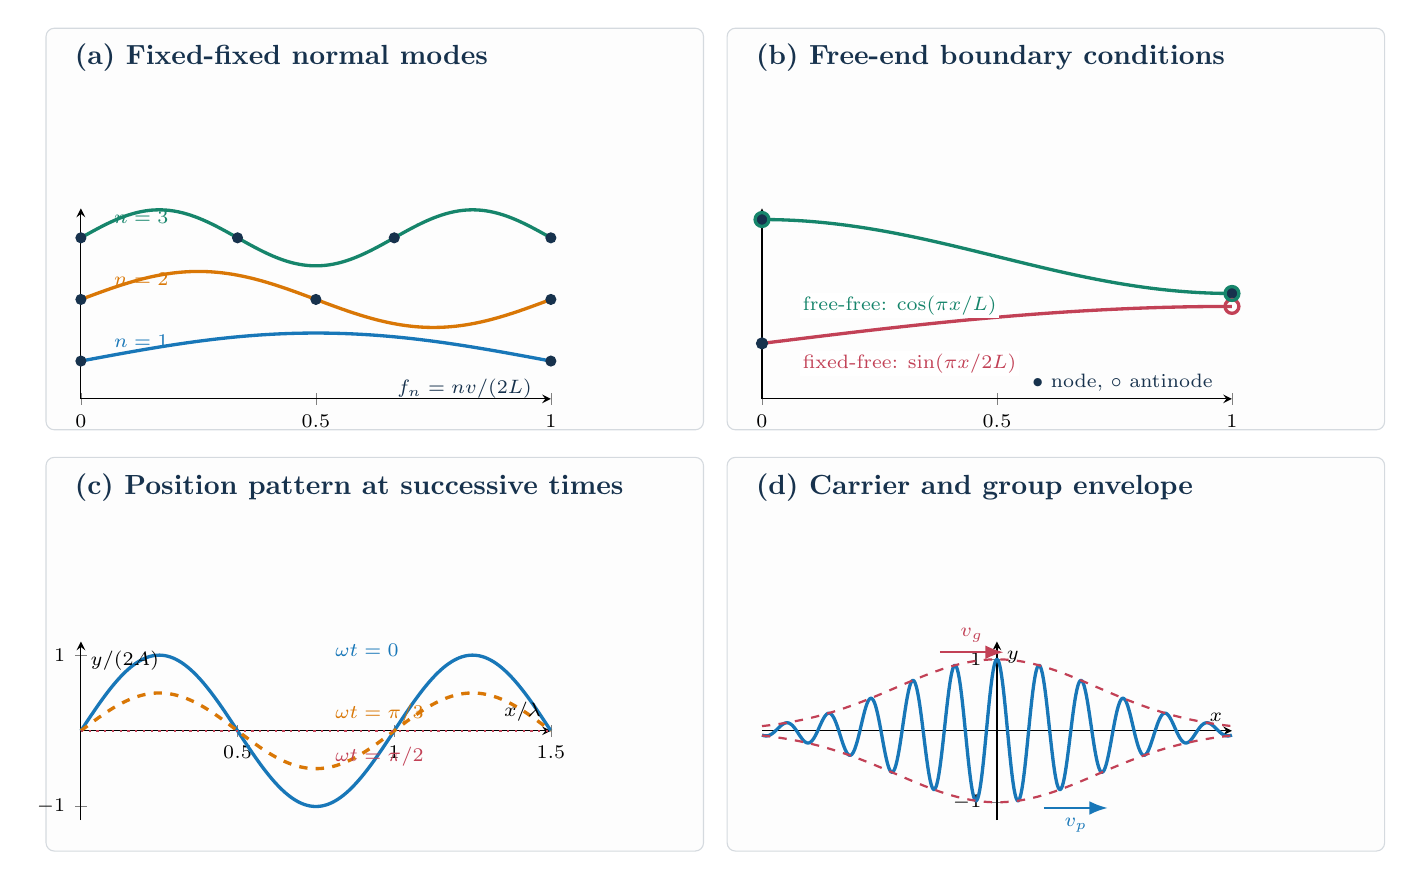
\begin{tikzpicture}[font=\small,>=Latex]
\tikzset{panel/.style={draw=ink!18,rounded corners=3pt,fill=ink!1}}

\node[panel,minimum width=8.35cm,minimum height=5.1cm,anchor=south west] at (0,5.35) {};
\node[font=\bfseries,ink,anchor=west] at (.25,10.08) {(a) Fixed-fixed normal modes};
\begin{axis}[at={(.45cm,5.75cm)},anchor=south west,width=7.55cm,height=4.0cm,
  axis lines=left,xmin=0,xmax=1,ymin=-1.35,ymax=5.45,
  xtick={0,.5,1},ytick=\empty,tick label style={font=\scriptsize},label style={font=\scriptsize},clip=false]
  \addplot[blue,very thick,domain=0:1,samples=160]{sin(deg(pi*x))};
  \addplot[orange,very thick,domain=0:1,samples=160]{2.2+sin(deg(2*pi*x))};
  \addplot[green,very thick,domain=0:1,samples=160]{4.4+sin(deg(3*pi*x))};
  \addplot[only marks,mark=*,mark size=1.8pt,ink] coordinates {(0,0)(1,0)(0,2.2)(.5,2.2)(1,2.2)(0,4.4)(.3333,4.4)(.6667,4.4)(1,4.4)};
  \node[blue,font=\scriptsize,anchor=west] at (axis cs:.05,.72) {$n=1$};
  \node[orange,font=\scriptsize,anchor=west] at (axis cs:.05,2.92) {$n=2$};
  \node[green,font=\scriptsize,anchor=west] at (axis cs:.05,5.12) {$n=3$};
  \node[ink,font=\scriptsize,anchor=east] at (axis cs:.98,-1.0) {$f_n=nv/(2L)$};
\end{axis}

\node[panel,minimum width=8.35cm,minimum height=5.1cm,anchor=south west] at (8.65,5.35) {};
\node[font=\bfseries,ink,anchor=west] at (8.90,10.08) {(b) Free-end boundary conditions};
\begin{axis}[at={(9.10cm,5.75cm)},anchor=south west,width=7.55cm,height=4.0cm,
  axis lines=left,xmin=0,xmax=1,ymin=-1.5,ymax=3.65,
  xtick={0,.5,1},ytick=\empty,tick label style={font=\scriptsize},label style={font=\scriptsize},clip=false]
  \addplot[red,very thick,domain=0:1,samples=160]{sin(deg(pi*x/2))};
  \addplot[green,very thick,domain=0:1,samples=160]{2.35+cos(deg(pi*x))};
  \addplot[only marks,mark=*,mark size=2pt,ink] coordinates {(0,0)(0,3.35)(1,1.35)};
  \addplot[only marks,mark=o,mark size=2.5pt,very thick,red] coordinates {(1,1)};
  \addplot[only marks,mark=o,mark size=2.5pt,very thick,green] coordinates {(0,3.35)(1,1.35)};
  \node[red,font=\scriptsize,anchor=west,fill=white,inner sep=1pt] at (axis cs:.08,-.55) {fixed-free: $\sin(\pi x/2L)$};
  \node[green,font=\scriptsize,anchor=west,fill=white,inner sep=1pt] at (axis cs:.08,1.02) {free-free: $\cos(\pi x/L)$};
  \node[ink,font=\scriptsize,anchor=east] at (axis cs:.98,-1.05) {$\bullet$ node, $\circ$ antinode};
\end{axis}

\node[panel,minimum width=8.35cm,minimum height=5.0cm,anchor=south west] at (0,0) {};
\node[font=\bfseries,ink,anchor=west] at (.25,4.62) {(c) Position pattern at successive times};
\begin{axis}[at={(.45cm,.4cm)},anchor=south west,width=7.55cm,height=3.85cm,
  axis lines=middle,xlabel={$x/\lambda$},ylabel={$y/(2A)$},xmin=0,xmax=1.5,ymin=-1.18,ymax=1.18,
  xtick={0,.5,1,1.5},ytick={-1,0,1},tick label style={font=\scriptsize},label style={font=\scriptsize},clip=false]
  \addplot[blue,very thick,domain=0:1.5,samples=180]{sin(deg(2*pi*x))};
  \addplot[orange,very thick,dashed,domain=0:1.5,samples=180]{.5*sin(deg(2*pi*x))};
  \addplot[red,thick,dotted,domain=0:1.5,samples=2]{0};
  \node[blue,font=\scriptsize,anchor=south west] at (axis cs:.78,.85) {$\omega t=0$};
  \node[orange,font=\scriptsize,anchor=north west] at (axis cs:.78,.48) {$\omega t=\pi/3$};
  \node[red,font=\scriptsize,anchor=north west] at (axis cs:.78,-.08) {$\omega t=\pi/2$};
\end{axis}

\node[panel,minimum width=8.35cm,minimum height=5.0cm,anchor=south west] at (8.65,0) {};
\node[font=\bfseries,ink,anchor=west] at (8.90,4.62) {(d) Carrier and group envelope};
\begin{axis}[at={(9.10cm,.4cm)},anchor=south west,width=7.55cm,height=3.85cm,
  axis lines=middle,xlabel={$x$},ylabel={$y$},xmin=-7,xmax=7,ymin=-1.25,ymax=1.25,
  xtick=\empty,ytick={-1,0,1},tick label style={font=\scriptsize},label style={font=\scriptsize},clip=false]
  \addplot[blue,very thick,domain=-7:7,samples=650]{exp(-x^2/18)*cos(deg(5*x))};
  \addplot[red,thick,dashed,domain=-7:7,samples=180]{exp(-x^2/18)};
  \addplot[red,thick,dashed,domain=-7:7,samples=180]{-exp(-x^2/18)};
  \draw[->,red,thick] (axis cs:-1.7,1.1)--(axis cs:.2,1.1) node[midway,above,font=\scriptsize] {$v_g$};
  \draw[->,blue,thick] (axis cs:1.4,-1.08)--(axis cs:3.3,-1.08) node[midway,below,font=\scriptsize] {$v_p$};
\end{axis}
\end{tikzpicture}
\end{document}
